\chapter{Introduction to Change-based Model Persistence}
We present an approach for change-based (as opposed to state-based) model persistence that can facilitate high-performance incremental model processing (e.g. validation, transformation) by minimising the cost of change identification when models evolve. We illustrate a prototype that implements the proposed approach on top of the Eclipse Modelling Framework and we present a roadmap for further work in this direction.

\section{Introduction}
\label{Introduction}
% The way we handle models nowadays are mostly based on non-incremental approach -- it persists states of models as snapshots. When the size of a model is small, the cost to process (e.g. validate, transform) the model is insignificant. Once the model becomes large, the processes turn to be cumbersome, particularly when small changes are made, but the whole model needs to be re-validated and re-transformed. To overcome this issue, several existing works \cite{egyed2011automatically, jouault2010towards, rath2012derived, ogunyomi2015property} have applied variants of incremental-based approach to improving model operation performance. The ``incremental" means the time to update the results of a model processing operation should be proportional to the size of the change of a modified model. This research aims to persist models change history as a mean to harness incremental-based approach to enable high-performance model processing operations.

% As MBSE is used for the development of larger and more complex systems in a variety of domains, the ability to process (e.g. validate, transform, generate code from) large models in an incremental fashion as they evolve becomes essential. ``Incremental'' in this context means that the amount of time it takes to update the results of a model processing operation on a modified model, is generally proportional to the size of the change, as opposed to the size of the model.

To reap the benefits of Model-Based Software Engineering in the context of large and complex systems, the ability to process large models in an incremental fashion as they evolve is essential. Current incremental model processing techniques only deliver limited performance benefits due to slow and imprecise model change detection capabilities or are limited to a single-developer environment; not realistic for real-world software development projects.

The research introduced in this paper aims at enabling flexible and high-performance incremental model processing through change-based model persistence. That is, instead of persisting snapshots of the state of models, we propose turning models inside out and persisting their change history. The proposed approach has the potential to deliver step-change performance benefits in incremental model processing, as well as a wide range of other benefits and novel capabilities.

The rest of the paper is structured as follows. Section \ref{sec:the_key_challenge_of_ _incrementality} reviews the key-challenge of incrementality in MBSE. Section \ref{sec:identifying_changes_in models} provides an overview of existing approaches for identifying changes in models. Section \ref{sec:proposed_approach} overviews our proposed approach and Section \ref{sec:prototype_implementation} discusses our prototype implementation on top of the Eclipse Modelling Framework. The potential benefits and novel capabilities, as well as the challenges of change-based model persistence, are presented in Sect. \ref{sec:benefits_and_novel_capabilities} and Sect. \ref{sec:challenges_and_future_works} respectively. Section \ref{sec:evaluation_strategy} presents our evaluation strategy and Sect. \ref{sec:conclusions} concludes this paper.

\section{The Key-Challenge of Incrementality}
\label{sec:the_key_challenge_of_ _incrementality}
%\dk{See \url{https://en.wikibooks.org/wiki/LaTeX/Labels_and_Cross-referencing} for naming conventions for LaTeX labels}
To illustrate the concept of incrementality, a contrived running example is used where after every modification to an organisational chart model (see Fig. \ref{fig:initial_chart}), the model needs to be:

\begin{itemize}
    \item Validated against a domain-specific constraint (that no employee directly manages more than 7 other employees).
    \item Transformed into a number of employee reports (plain text files, one for each employee) through a model-to-text transformation. Each report should contain the name of the employee, and the names of her direct subordinates.
\end{itemize}

Figures \ref{fig:initial_chart} and \ref{fig:modified_chart} are two consecutive versions of a sample organisational chart model. When the validation constraint is evaluated against the first version of the model (Fig. \ref{fig:initial_chart}), it verifies that all three employees manage fewer than 7 other employees, and the model-to-text transformation then produces three text files that correspond to the employees in the model. In the sequel, in Fig. \ref{fig:modified_chart}, the model is updated to reflect that a new employee has been hired (Richmond) under the management of Jen. 

\begin{figure}[b!]
    \centering
    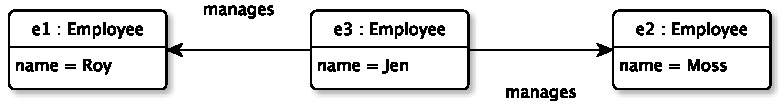
\includegraphics[width=\linewidth]{initial_chart}
    \caption{Initial version of the organisational chart model.}
    \label{fig:initial_chart}
\end{figure}

\begin{figure}[b!]
    \centering
    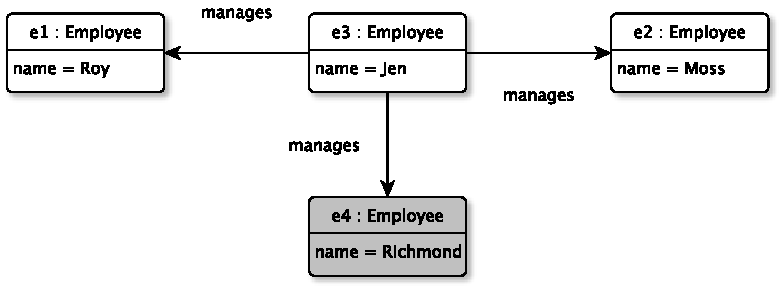
\includegraphics[width=\linewidth]{modified_chart}
    \caption{Modified version of the organisational chart model of Fig. \ref{fig:initial_chart}.}
    \label{fig:modified_chart}
\end{figure}

A non-incremental model validation engine would treat the model of Fig. \ref{fig:modified_chart} as if it was a new model and would evaluate the constraint above against every employee in the model. An incremental model validation engine, on the other hand, would identify that the previously established satisfaction of the constraint for employees Moss and Roy cannot have been possibly compromised by the changes made, and would only re-evaluate the constraint for Jen and Richmond instead. 

Similarly, a non-incremental model-to-text transformation would generate and overwrite all employee reports from scratch. On the contrary, an incremental model-to-text transformation, would identify that it only needs to generate a new report for the new employee (Richmond), and to recompute and overwrite the contents of Jen's report (as she is now managing an additional employee)---but not the reports of Moss or Roy, as these cannot have been affected by the changes made to the model.

While the overhead of executing transformations and validation constraints on small models like the one in Fig. \ref{fig:modified_chart} is negligible, non-incremental execution can become a significant bottleneck for large evolving models. As stressed in Selic's seminal work \cite{selic2003pragmatics}, with reference to model-to-text transformation, ``... \emph{this is particularly true in the latter phases of the development cycle when programmers make many small changes as they fine-tune the system. To keep this overhead low, it is crucial for the code generators to have sophisticated change impact analysis capabilities that minimize the amount of code regeneration}".

As demonstrated by the pioneering work of Egyed \cite{egyed2011automatically}, to achieve incremental re-execution of (deterministic) queries on structured models, an execution engine needs to:

\begin{enumerate}
    \item Record model element property accesses during the initial execution of the queries;
    \item Identify new and deleted elements and modified model element properties in the new version of the model;
    \item Combine the information collected in the steps above to identify the subset of (potentially) affected rules/queries/templates that need to be re-executed.
\end{enumerate}

To illustrate this, we use an OCL implementation of the domain-specific constraint in List. \ref{lst:constraint}.

\begin{lstlisting}[style=ocl,caption={OCL constraint requiring that no employee directly manages more than 7 other employees.},label=lst:constraint]
context Employee
inv NoMoreThan7: self.manages->size() <= 7
\end{lstlisting}

During the initial evaluation of the constraint on the model of Fig. \ref{fig:initial_chart}, an incremental OCL engine would compute the property access trace displayed in Table \ref{tab:property_access_trace} as a side-product. Now, when the model is updated (Fig. \ref{fig:modified_chart}), the execution engine can identify that:

\begin{table}[b]
    \centering
    \caption{Property-access trace of the evaluation of the constraint in List. \ref{lst:constraint} on the model of Fig. \ref{fig:initial_chart}.}
    \begin{tabular}{p{4.8cm} p{2.1cm} p{2cm} p{2.1cm}}
        \hline 
        \textbf{Constraint} & \textbf{Context} & \textbf{Accessed Element} & \textbf{Accessed Property} \\ 
        \hline 
        \emph{Employee.NoMoreThan7}  & \emph{e1} & \emph{e1} & \emph{manages} \\ 
        \emph{Employee.NoMoreThan7}  & \emph{e2} & \emph{e2} & \emph{manages} \\ 
        \emph{Employee.NoMoreThan7}  & \emph{e3} & \emph{e3} & \emph{manages} \\ 
        \hline 
    \end{tabular} 
    \label{tab:property_access_trace}
\end{table}

\begin{itemize}
    \item There is new element in the model (\emph{e4} - Richmond) for which the constraint has not been evaluated;
    \item The value of the manages property of Jen (\emph{e3}) has changed, and as such, it needs to re-evaluate the constraint on this model-element.
\end{itemize}

Egyed has shown that the property-access recording approach is applicable to queries of arbitrary complexity, as long as they are deterministic. More recent work has shown that variants of this approach can be used to achieve incrementality in a wide range of model processing operations, including model-to-model transformation \cite{jouault2010towards}, model-to-text transformation \cite{ogunyomi2015property}, model validation, and pattern matching \cite{rath2012derived}---as long as changes to models can be precisely identified (step 2 in the list above).

\section{Identifying Changes in Models}
\label{sec:identifying_changes_in models}
There are two approaches in the literature for identifying changes in models in order to enable incremental re-execution of model processing operations.

\textbf{Notifications}. In this approach, the incremental execution engine needs to hook into the notification facilities provided by the modelling tool through which the developer edits the model, so that the engine can directly receive notifications as soon as changes happen (e.g. a new employee (\emph{e4}) has been added, the name property of employee \emph{e4} has been changed to ``Richmond"). This is an approach taken by the IncQuery incremental pattern matching framework \cite{rath2012derived} and the ReactiveATL incremental model-to-model transformation engine \cite{ogunyomi2015property}. The main advantage of this approach is that precise and fine-grained change notifications are provided for free by the modelling tool (and thus do not need to be computed by the execution engine---which as discussed below can be expensive and inefficient). On the downside, this approach is a poor fit for collaborative development settings where modelling and automated model processing activities are performed by different members of the team.

\textbf{Model Differencing}. This approach eliminates the coupling between modelling tools and incremental execution engines. Instead of depending on live notifications, in this approach the developer in charge of automated model processing, needs to have access to a copy of the last version of the model that the model processing program (e.g. the model-to-text transformation) was executed upon, so that it can be compared against the current version of the model (e.g. using a model-differencing framework such as SiDiff or EMFCompare) and the delta can be computed on demand. The main advantage of this approach is that it works well in a collaborative development environment where typically developers have distinct roles and responsibilities. On the downside, model comparison and differencing are computationally expensive and memory-greedy (both versions of the model need to be loaded into memory before they can be compared), thus largely undermining the time and resource saving potentials of incremental re-execution. This approach is adopted by the Xpand model-to-text transformation language. According to the developers of the language, using this approach, a speed-up of only around 50\% is observed compared to non-incremental transformation\footnote{\url{http://wiki.eclipse.org/Xpand/New_And_Noteworthy\#Incremental_Generation}}, which is consistent with our experience from using Xpand.

In summary, incremental model processing currently delivers significant performance benefits only in a single-developer environment where the modeller is also responsible for performing all the (incremental) model processing operations. As a result, in collaborative development environments, developers need to either forgo incremental model processing altogether or to work around this limitation by manually steering model processing programs to process only subsets of their models, which is cumbersome and error prone.

\begin{lstlisting}[style=xmi,caption={State-based representation of the model of Figure \ref{fig:modified_chart} in (simplified) XMI.},label=lst:xmimodel]
<Employee xmi:id="e2" name="Jen">
<manages xmi:id="e1" name="Roy"/>
<manages xmi:id="e3" name="Moss"/>
<manages xmi:id="e4" name="Richmond"/>
</Employee>
\end{lstlisting}


\begin{lstlisting}[style=xml,caption={Change-based representation of the model of Figure \ref{fig:modified_chart}.},label=lst:cbpmodel]
<session id="s1"/>
<create eclass="Employee" epackage="employee" id="0"/>
<add-to-resource position="0"><value eobject="0"/></add-to-resource>
<set-eattribute name="name" target="0"><value literal="Roy"/></set-eattribute>
<create eclass="Employee" epackage="employee" id="1"/>
<add-to-resource position="1"><value eobject="1"/></add-to-resource>
<set-eattribute name="name" target="1"><value literal="Jen"/></set-eattribute>
<create eclass="Employee" epackage="employee" id="2"/>
<add-to-resource position="2"><value eobject="2"/></add-to-resource>
<set-eattribute name="name" target="1"><value literal="Moss"/></set-eattribute>
<remove-from-resource><value eobject="0"/></remove-from-resource>
<add-to-ereference name="manages" position="0" target="1"><value eobject="0"/></add-to-ereference>
<remove-from-resource><value eobject="2"/></remove-from-resource>
<add-to-ereference name="manages" position="1" target="1"><value eobject="2"/></add-to-ereference>
<session id="s2"/>
<create eclass="Employee" epackage="employee" id="3"/>
<add-to-resource position="1"><value eobject="3"/></add-to-resource>
<set-eattribute name="name" target="3"><value literal="Richmond"/></set-eattribute>
<remove-from-resource><value eobject="3"/></remove-from-resource>
<add-to-ereference name="manages" position="2" target="2"><value eobject="3"/></add-to-ereference>
\end{lstlisting}

\section{Proposed Approach}
\label{sec:proposed_approach}
The ambition of this research is to enable high-performance incremental model management in collaborative software development environments by challenging one of the fundamental assumptions of contemporary modelling frameworks and tools: as opposed to persisting snapshots of the state of models (which is what virtually all modelling tools and frameworks currently do), we propose turning models inside out and persisting their change history instead.

To illustrate the proposed approach, List. \ref{lst:xmimodel} shows a state-based representation of the model of Fig. \ref{fig:modified_chart} in (simplified) XMI, and List. \ref{lst:cbpmodel} shows the proposed equivalent change-based representation of the same model. Instead of a snapshot of the state of the model, the representation of List. \ref{lst:cbpmodel} captures the complete sequence of change events (create/set/add/remove/delete) that were performed on the model since its creation, organised in editing sessions (2 editing sessions in the case of this model). Replaying these changes produces the same state as the one captured in List. \ref{lst:xmimodel}, so the proposed representation carries at least as much information as the state-based representation.

Such a representation is particularly suitable for incremental model processing. For example, if the model-to-text transformation discussed above ``remembers" that in its previous invocation it had processed up to editing session \emph{s1} of the model, it can readily identify the changes that have been made to the model since then (i.e. in session \emph{s2} –- lines 15-20) instead of having to rediscover them through (expensive) state-based model differencing.

\section{Prototype Implementation}
\label{sec:prototype_implementation}
We have implemented a prototype\footnote{The prototype is available under \url{https://github.com/epsilonlabs/emf-cbp}.} of the change-based model persistence format using the notification facilities provided by the Eclipse Modelling Framework. In our implementation we use a subclass of EMF's \emph{EContentAdapter} (\emph{ChangeEventAdapter}) to receive and record \emph{Notification} events produced by the framework for every model-element level change.

\begin{figure}[th]
    \centering
    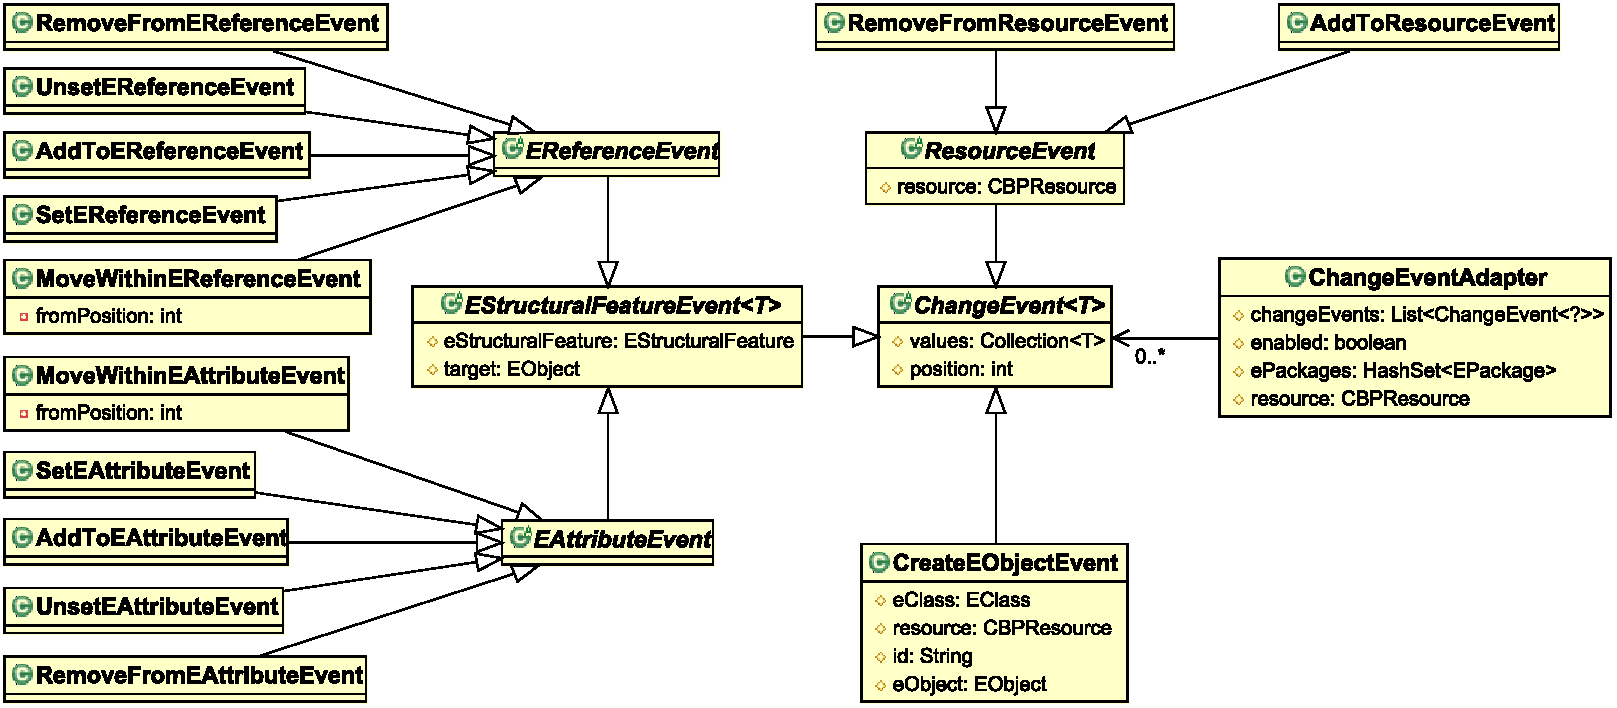
\includegraphics[scale=0.32]{events}
    \caption{Event classes to represent changes of models.}
    %\dk{It would be useful to redraw the diagram so that important properties are visible (e.g. an AddToEReference event has an ``index'' and a ``value'') and also to discuss events - particularly those that may not immediately make sense to the reader (e.g. AddToResourceEvent, RegisterEPackageEvent)}
    \label{fig:events}
\end{figure}

Since not all change events are relevant to change-based persistence (e.g. EMF also produces change notifications when listeners/adapted are added/removed from the model), we have defined a set of event classes to represent events of interest. The event classes are depicted in Fig. \ref{fig:events} as subclasses of the \emph{ChangeEvent} abstract class.  %In Fig. \ref{events}, unlike other event classes,\emph{RegisterEPackageEvent} class has a reference to \emph{ChangeEventAdapater} class since the \emph{RegisterEPackageEvent} holds the information of \emph{EPackage}'s name (List. \ref{cbpmodel1}, line 3) required by the \emph{ChangeEventAdapter} to recreate a model in a de-serialisation process. 

The \emph{ChangeEvent} class has a mutli-valued \emph{values} attribute which can accommodate both single-valued (e.g. set/add) or mutli-valued events (e.g. addAll/removeAll). \emph{ChangeEvent} can also accommodate different types of values, such as \emph{EObject}s for \emph{EReferenceEvents}, and primitive values (e.g. Integer, String) for \emph{EAttributeEvents}. The \emph{ChangeEvent} class also has a position attribute to hold the  index of an \emph{EObject} or a literal when they are added to a \emph{Resource}, \emph{EReference}, or \emph{EAttribute} with multiple values (Lst. \ref{lst:cbpmodel}, line 3, 6, 9, 12, 14, 17, 20). 

%When an event happens, it can involve multiple instances of \emph{EObject}. In  Lst. \ref{lst:cbpmodel} line 21, when \emph{e4} is added as an employee that \emph{e2} manages (\emph{AddToEReferenceEvent}), the \emph{e4}, \emph{manages}, and \emph{e2} are set as the event's \emph{value}, \emph{eStructuralFeature} (in this case \emph{name}), and \emph{target} respectively. The \emph{eStructuralFeature} and \emph{target} attributes are defined in the \emph{EStructuralFeatureEvent} class, which are inherited by \emph{EReferenceEvent} and \emph{EAttributeEvent} and all their subclasses (Fig. \ref{fig:events}).  

% The \emph{RegisterEPackageEvent} class is responsible to capture an event when the EMF's \emph{EPackage} of a model is registered to the \emph{ChangeEventAdapter}'s \emph{ePackages} attribute (Fig. \ref{fig:events} and Lst. \ref{lst:cbpmodel}, line 2). The information of the \emph{EPackage} is required in further model creation (e.g. create model from XML-formatted representation). The \emph{ChangeEventAdapter}'s is designed to handle multiple packages of models.

Every time an \emph{EObject} is added to the model, a \emph{CreateEObjectEvent} and an \emph{AddToResourceEvent} are recorded (lines 2-3, 5-6, 8-9, and 16-17 in Lst. \ref{lst:cbpmodel}). When an EObject is deleted, or moved to a containment \emph{EReference} deeper in the model (Lst. \ref{lst:cbpmodel}, line 12, 14, 20), a \emph{RemoveFromResourceEvent} (Lst. \ref{lst:cbpmodel}, line 11, 13, 19) is recorded.

The \emph{ChangeEventAdapter} receives EMF change notifications in its \emph{notifyChanged()} method and filters and transforms them into appropriate change events. As an example of how notifications are filtered and transformed, Listing \ref{lst:javacode} shows how we handle \emph{Notification.UNSET} events based on the type of the changed feature i.e. an \emph{UnsetEAttributeEvent} is instantiated if the feature of the notifier is an \emph{EAttribute}, or an \emph{UnsetEReferenceEvent}  is created if the notifier is an \emph{EReference}. The transformed instances are then stored into a list of events in \emph{ChangeEventAdapter} (\emph{changeEvents}) for persistence. 

\begin{lstlisting}[style=java,caption={Simplified Java code to handle notification events.},label=lst:javacode]
public class ChangeEventAdapter extends EContentAdapter {
...
@override
public void notifyChanged(Notification n) {
...
switch (n.getEventType()) {
... // other events
case Notification.UNSET: {
if (n.getNotifier() instanceof EObject) {
EStructuralFeature feature = (EStructuralFeature) n.getFeature();
if (feature instanceof EAttribute) {
event = new UnsetEAttributeEvent();
} else if (feature instanceof EReference) {
event = new UnsetEReferenceEvent();
}
} break;
} 
... // other events
\end{lstlisting}	

To integrate seamlessly with the EMF framework and to eventually support multiple concrete change-based serialisation formats (e.g. XML-formatted representation for readability and binary for performance/size), we have created the \emph{CBPResource} abstract class, that extends EMF's built-in \emph{ResourceImpl} class. The role of the abstract class is to encapsulate all change recording functionality while the role of its concrete subclasses is to implement serialisation and de-serialisation. For example, \emph{CBPXMLResourceImpl} persists changes in a line-based format where every change is serialised as a single-line XML document. In this way, when a model changes, we can append the new changes to the end of the model file without needing to serialise the entire model again. We have also implemented a \emph{CBPXMLResourceFactory} class that extends EMF's \emph{ResourceFactoryImpl}, as the factory class for change-based models. Figure \ref{fig:resources} shows the relationships between these classes.

%The \emph{CBPXMLResourceImpl} uses an instance of \emph{ChangeEventAdapater} class to obtain a list of change events. The relationships of these classes are depicted in Fig. \ref{fig:resources}. By overriding \emph{CBPResource}'s \emph{doSave} and  \emph{doLoad} methods, we can perform serialization of the event list into an XML-formatted file and load it back again later. The representation is not a valid, complete XML format since it has no root node. Instead, it is a list of XML-formatted lines so that changes can be saved by appending new lines to the file to improve performance.


\begin{figure}[th]
    \centering
    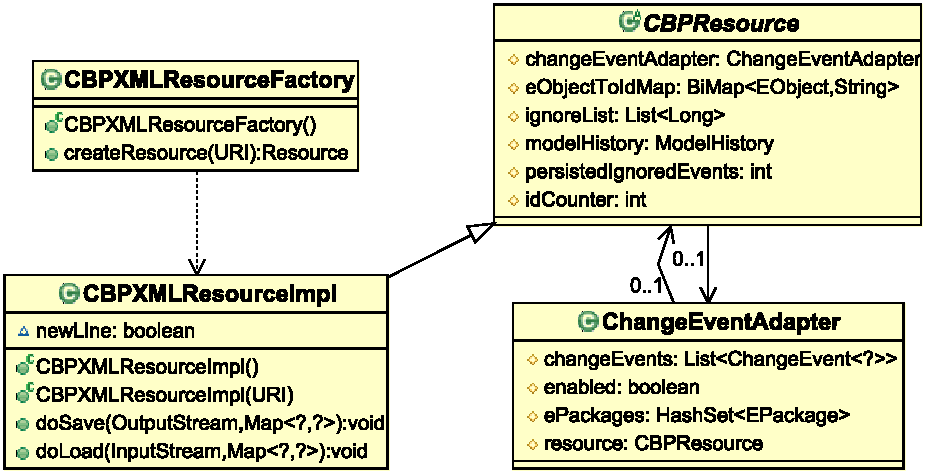
\includegraphics[scale=0.32]{resources}
    \caption{Factory, resources, and ChangeEventAdapter classes.}
    %\dk{See previous comment on redrawing. In its current form the diagram can be interpreted as stating that a CBPXMLResourceFactory ``has a'' CBPXMLResourceImpl, which is incorrect.}
    \label{fig:resources}
\end{figure}

\section{Benefits and Novel Capabilities}
\label{sec:benefits_and_novel_capabilities}
Beyond facilitating incremental processing, the proposed representation also has the potential to deliver a wide range of benefits and novel capabilities, compared to the currently prevalent state-based representations, some of which are discussed below.

\begin{itemize}
    \item With appropriate tool support, modellers will be able to ``replay" (part of) the change history of a model (e.g. to understand design decisions made by other developers, for training purposes). In state-based approaches, this can be partly achieved if models are stored in a version-control repository (e.g. Git). However, the granularity would only be at the commit level.
    \item By analysing models serialised in the proposed representation, modelling language and tool vendors will be able to develop deeper insights into how modellers actually use these languages/tools in practice and utilise this information to guide the evolution of the language/tool.
    \item By attaching additional information to each session (e.g. the id of the developer, references to external documents/URLs), sequences of changes can be traced back to the developer that made them, or to requirements/bug reports that triggered them.
    \item Persisting changes to large models after an editing session will be significantly faster compared to serialising the entire state of the model, as only changes made during the session will need to be appended to the model file.
    \item The performance and precision of model comparison and merging can be substantially improved, particularly for large models with shared editing histories.
\end{itemize}

\section{Challenges and Future Work}
\label{sec:challenges_and_future_works}
The proposed approach also comes with a number of challenges that this research will need to overcome.

\textbf{Loading Overhead}. While, as discussed above, persisting changes to large models is expected to be much faster and resource-efficient compared to state-based approaches, loading models into memory by naively replaying the entire change history is expected to have a significant overhead. To address this challenge, we will develop dedicated algorithms and data structures that will reduce the cost of change-based model loading (e.g. by recording and ignoring events -- events that are later overridden or cancelled out by other events). 

\textbf{Fast-Growing Model Files}. Persisting models in a change-based format means that model files will keep growing in size during their evolution significantly faster than their state-based counterparts. To address this challenge, (1) we will propose sound change-compression operations (e.g. remove older/unused information) that can be used to reduce the size of a model in a controlled way. (2) We will develop a compact textual format that will minimise the amount of space required to record a change (a textual line-separated format is desirable to maintain compatibility with file-based version control systems). (3) We will propose a hybrid model persistence format which will be able to incorporate both change-based and state-based information. 

\section{Evaluation Strategy}
\label{sec:evaluation_strategy}
The findings of the research will be evaluated in the small in the context of the tasks in which they will be developed, and in the large through industrial case studies. For the first type of evaluation (in the small), where there are existing approaches that the algorithms and tools developed in this research seek to outperform (e.g. change-based incremental validation vs. state-based incremental validation), comparative evaluation will be conducted to assess the benefits and limitations of our approaches. For algorithms and tools that have no direct competitors in the literature, their contributions will be assessed in comparison to the baseline they seek to improve (e.g. in this case, persisting full change histories). Evaluation in the large will be conducted through appropriate case studies in collaboration with industrial peers.

\section{Conclusions}
\label{sec:conclusions}
Through turning models inside out and persisting their change history, this research aims at enabling high-performance incremental model processing in collaborative development settings. The proposed approach also has the potential to enable model analytics, more fine-grained tracing and to improve the precision and performance of model comparison and merging. A prototype implementation of a change-based persistence format has been presented, the main envisioned challenges have been listed and an evaluation strategy has been outlined. %Several future works also have been defined to tackle the identified challenges in realising the change-based model. Comparative evaluation will be conducted to assess the benefits and limitation of our approaches by comparing them to existing algorithms, tools, or baselines that they seek to improve.
